\documentclass[12pt,letterpaper,final]{report}
\usepackage[utf8]{inputenc}
\usepackage{amsmath}
\usepackage{amsfonts}
\usepackage{amssymb}
\usepackage{amsthm}
\renewcommand\qedsymbol{$\blacksquare$}
\usepackage{enumerate}
\usepackage{hyperref}
\usepackage{pdfpages}
\usepackage{graphics}
\usepackage{graphicx}
\usepackage{tikz}
\usepackage{tikz-qtree}
\usetikzlibrary{automata,arrows}
\usepackage[
  backend=biber,
  style=authoryear,
  sorting=nyt          % sort by name, year, title
]{biblatex}
\addbibresource{references.bib}

% \author{Marius Zimand}
\author{Jonathan Llovet}

\begin{document}

\fbox{
  \vbox{
    \begin{flushleft}
      Jonathan Llovet \\  % authors' names
      COSC 417 \\  %class
      2026-02-19, 11:59 PM (EST) \\  % date
    \end{flushleft}
    \center{\Large{\textbf{Assignment 2}}}
    %\end{mdframed}
  } % end vbox
} % end fbox
\vline

Do (or at least sketch the solutions) without turning in anything the following exercises from the textbook: 1.4 (a-d), 1.5 (a-d), 1.6(a-d), 1.7(a-d).

\medskip

{\bf Problem 1.}  The formal description of a DFA $M$ is $(\{q_1, q_2, q_3, q_4, q_5\}, \{u,d\}, \delta , q_3, \{q_3\})$, where  $\delta$ is given by the following table. Draw the state diagram (i.e.\,  the graph representation) of this machine.
\smallskip

\begin{tabular}{|l|ll|}
  \hline
         & $u$    & $d$   \\
  \hline
  $q_1$  & $q_1$  & $q_2$ \\
  $q_2 $ & $q_1$  & $q_3$ \\
  $q_3$  & $q_2 $ & $q_4$ \\
  $q_4$  & $q_3$  & $q_5$ \\
  $q_5$  & $q_4$  & $q_5$ \\
  \hline
\end{tabular}
\smallskip


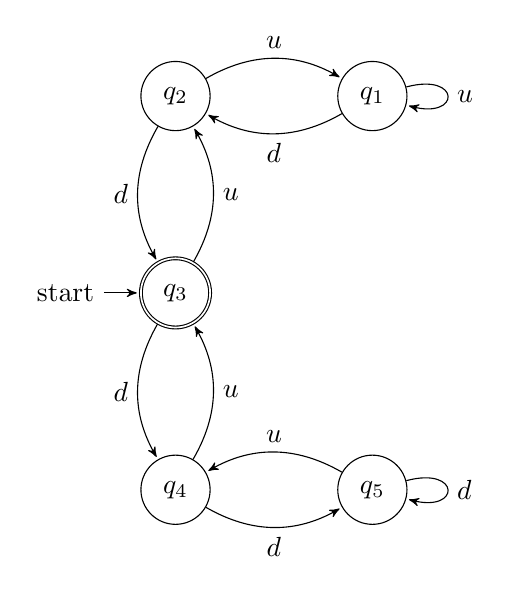
\begin{tikzpicture}[>=stealth',shorten >=1pt,auto,node distance=2.5cm]

  \node[initial, state, accepting] (3) {$q_{3}$};
  \node[state] (2) [above of=3] {$q_{2}$};
  \node[state] (1) [right of=2] {$q_{1}$};
  \node[state] (4) [below of=3] {$q_{4}$};
  \node[state] (5) [right of=4] {$q_{5}$};

  \path[->]
  (1) edge [loop right] node {$u$} (1)
  (1) edge [bend left] node[below] {$d$} (2)

  (2) edge [bend left] node[above] {$u$} (1)
  (2) edge [bend right] node[left] {$d$} (3)

  (3) edge [bend right] node[right] {$u$} (2)
  (3) edge [bend right] node[left] {$d$} (4)

  (4) edge [bend right] node[right] {$u$} (3)
  (4) edge [bend right] node[below] {$d$} (5)
  
  (5) edge [bend right] node[above] {$u$} (4)
  (5) edge [loop right] node {$d$} (5)
  ;
\end{tikzpicture}

\medskip

Show the computation done by this machine on input $uddu$ (i.e., the sequence of states it enters; see Example 1.17 in the textbook).

The sequence of states the DFA above enters when computing the string $uddu$ is
$q_3, q_2, q_3, q_4, q_3$

\medskip

{\bf Problem 2.}	 	Give the state diagram of DFAs with the specified number of states (or less) for each of the following languages over the alphabet $\{0,1\}$.
\begin{enumerate}

  \item[a.]	$\{w \mid w \mbox{ begins with a $1$ and ends with a $0$}\}$, DFA with $4$ states.  Show the computation (i.e., the sequence of states it enters; see Example 1.17 in the textbook) made by your DFA on input 10010 and on input 110011.

  \item[b.]	$\{w \mid w \mbox{ starts with $0$ and has odd length, or starts with $1$ and has even length}\}$, DFA with $3$ states. Show the computation (i.e., the sequence of states) made by your DFA on input 100101 and on input 11001.

  \item[c.]	$\{w \mid w \mbox{ does not contain the string 110}\}$, DFA  with $4$ states. Show the computation (i.e., the sequence of states) made by your DFA on input 1001101 and on input 1001.

        For each of the three DFA briefly and convincingly explain (give a ``common sense" explanation, I don't require a formal proof) why they accept the specified language.
\end{enumerate}
\medskip

{\bf Problem 3.}	 Give NFAs (in the form of state diagrams) with the specified number of states recognizing each the following languages. The alphabet is $\Sigma =\{0,1\}$.
\begin{enumerate}
  \item[a.]	$\{w \mid w \mbox{ ends with 00}\}$ with 3 states. Pick one input string that is in the language and one input string that is not in the language and show the two trees of computation possibilities made by your NFA on the two strings (as we did in class, see also Figure 1.29 in the textbook).

  \item[b.]	$\{w \mid w \mbox{ contains the substring 0101}\}$ with 5 states. Pick one input string that is in the language and one input string that is not in the language and show the two trees of computation possibilities made by your NFA on the two strings.
\end{enumerate}

As above, explain why your NFAs accept the corresponding language.
\bigskip

{\bf Problem 4.}	 For any string $w_1 w_2 \ldots w_n$, the reverse $w^R$  is the string $w$ in reverse order $w_n  \ldots w_2 w_1$.   For a language $A$, let $A^R = \{ w^R \mid w \mbox{ is in }A\}$ (in other words, $A^R$ consists of all the reverses of the strings in $A$).  Prove that if $A$ is regular, then $A^R$  is also regular. In your proof you have to  show how to convert a finite automaton for $A$ into a finite automaton for $A^R$.  Other arguments are possible, but will not give you the extra credit. (Note: Take care, an FA, whether deterministic or nondeterministic, has a single starting state).


\end{document}
